%
% File acl2014.tex
%
% Contact: koller@ling.uni-potsdam.de, yusuke@nii.ac.jp
%%
%% Based on the style files for ACL-2013, which were, in turn,
%% Based on the style files for ACL-2012, which were, in turn,
%% based on the style files for ACL-2011, which were, in turn, 
%% based on the style files for ACL-2010, which were, in turn, 
%% based on the style files for ACL-IJCNLP-2009, which were, in turn,
%% based on the style files for EACL-2009 and IJCNLP-2008...

%% Based on the style files for EACL 2006 by 
%%e.agirre@ehu.es or Sergi.Balari@uab.es
%% and that of ACL 08 by Joakim Nivre and Noah Smith

\documentclass[11pt]{article}
\usepackage{acl2014}
\usepackage{times}
\usepackage{url}
\usepackage{latexsym}
\usepackage{amsmath}
\usepackage{graphicx}

%\setlength\titlebox{5cm}

% You can expand the titlebox if you need extra space
% to show all the authors. Please do not make the titlebox
% smaller than 5cm (the original size); we will check this
% in the camera-ready version and ask you to change it back.


\title{Large-Scale Dataset Extraction by Semi-Supervised Learning}

\author{Jinfeng Rao\\
  Department of Computer Science \\
  University of Maryland \\
  {jinfeng@cs.umd.edu} \\\And
  Xing Niu \\
  Department of Computer Science \\
  University of Maryland \\
  {oxstar@cs.umd.edu} \\}

\date{}

\begin{document}
\maketitle
\begin{abstract}
%In some fields with no existing, widely-used benchmarks, finding appropriate datasets for experiments becomes a essential step in conducting research. Under these circumstances, a platform for storing dataset metadata, i.e, name, keyword, description, can be utilized for dataset inquiry and recommendation. 
In this paper, we leverage linguistic tools to solve the problem of dataset extraction from scientific literatures. We attempted three different approaches for extracting dataset from texts: classifier, dependency tree and conditional random fields(CRF). We evaluated these three approaches on a real world dataset, and got F1-Measure score higher as 70\%. Based on these work, we purposed a novel framework to extend conditional random fields in semi-supervised learning way by given a set of seeds(labeled datasets) as start point, and then iteratively find new datasets and patterns to bootstrap the learning process. The experiment results show the F1-Measure score continues increasing as the bootstrap process repeats.  
\end{abstract}
\section{Introduction}

Under such a situation, several dataset repositories have been developed and made public to researchers. For example, the KEEL\footnote{http://sci2s.ugr.es/keel/datasets.php} dataset repository and the UCI Machine Learning Repository\footnote{http://archive.ics.uci.edu/ml/} provide access to several hundred datasets in machine learning domain. The datasets in these repositories are most collected and maintained by manual work. However, collecting and integrating dataset sources mutually from the vast number of data sources, e.g, literatures, web, P2P sensor, is impractical. A more realistic scenario is to start with a small set of seed items( in this case, labeled datasets) and iteratively grow it by finding contextual patterns that extracts the set of seeds from the texts, then identify a larger set of seeds through the contextual patterns, finally pick the best subset of candidate seeds and add to previous seeds. This iterative learning process is called bootstrap or semi-supervised learning. In this paper, we first attempted three different approaches for extracting dataset from texts: classifier, dependency tree and conditional random fields. Then we purposed a novel bootstrapping framework for conditional random fields to guide the iterative learning process.  \\

In conclusion, our contributions includes,
\begin{itemize}
\item Compared with the very limited work in dataset extraction, we tried three different linguistic approaches to solve this problem, and the efficiency is verified by experiments on real-world data.
\item We purposed an original bootstrapping framework for conditional random fields, which includes an evaluation metric called \emph{feature contribution score} for measuring the contribution of this feature to find new contextual patterns, and an incremental training algorithm to avoid retraining of CRF in the iteratively learning process. 
\end{itemize}

\section{Related Work}
In this section, we first introduce some background knowledge in dependency tree and conditional random fields, then we discuss current work in the problem of dataset extraction.
\subsection{Dependency Tree}

\subsection{Conditional Random Fields}
Conditional Random Fields [] are probabilistic graph model assuming conditional probability $P(S|O)$ over designated output nodes $S$ given observed input node $O$. Unlike other approaches use the joint probability model $P(O,S)$, e.g, Hidden Markov Model [], the conditional nature of CRF results in the relaxation of the independence assumptions which is required by HMMs to obtain tractable inferences. More specifically, CRF can be viewed as a first-order markov chain globally conditioned on input nodes $O$. Each output state $S_i$ is viewed as a node in the graph model, which is conditioned on previous output node $S_{i-1}$ and input nodes $X$. \\

Let $o =\{o_1, o_2 ... o_n \}$ be the set of observed input data sequence, like a sequences of lines in the document. Let $S$ be the set of predicted states, each of which corresponds to a label (i.e, DATASET). Let $s = \{ s_1, s_2 ... s_n\}$ be some set of state sequence with any $s_i \in S$. CRF defines conditional probability of predicted state sequence given an input sequence as: 

\[
P(s | o,\lambda) = \frac{1}{Z_o} exp \left( \sum_{i}^n \sum_{k} \lambda_{k} f_{k}(s_{i-1}, s_{i}, o, i) \right)  \\
\]

where $Z_o$ is a normalization factor over all state sequence $S^n$, $f_{k}(s_{i-1}, s_{i}, o, i)$ is a feature function defined over its arguments, $\lambda_{k}$ is the learned weight for corresponding feature function $f_k$. Higher $\lambda_{k}$ represents its corresponding feature function more likely, thus feature function $f_k$ is more influential for predicting the state sequence. \\

To define feature functions, we construct a set of features $b(o, i)$ over the observed input sequence to express some characteristic of the empirical distribution of training data. An example of such feature is\\
\[
	b(o, i) = 
	\begin{cases}
		1, \text{if $o_i$ is in capitol form} \\
		0, \text{otherwise}
	\end{cases}
\]
Each feature function takes on the value of one of these real-valued features $b(o, i)$ if the current state and previous state takes particular values. For example, consider following feature function:
\[
	f_k(s_{i-1}, s_i, o, i) = 
	\begin{cases}
		b(o, i), &\text{if $s_{i-1} = DT$ and $s_{i} = DATASET$} \\
		0,	   &\text{otherwise}
	\end{cases}
\]
In fact, you can ask arbitrary questions(features) of the possible distribution over input sequence. We use $F_k(s, o) = \sum_{i}^n f_{k}(s_{i-1}, s_{i}, o, i)$ to sum the feature counts over input sequence and state sequence. Therefore, the conditional probability of predicted state sequence given an input sequence $P(s \| o, \lambda)$ can be rewritten as:
\[
	P(s | o, \lambda) = \frac{1}{Z_o} exp \left( \sum_{k} \lambda_{k} F_k(s, o) \right)
\]

The set of weights $\{ \lambda_k \}$ are trained to maximize the likelihood estimation of conditional probability $P(s | o, \lambda)$. Given the training data $\{(o^j, s^j)\}$, the objective function is:
\[
	L = \sum_{j} \log P(s^j | o^j, \lambda) -\sum_k \frac{\lambda_k^2}{2 \sigma^2} 
\]
where the second sum is the Gaussian priors over the set of weights $\{ \lambda_k \}$. Since the function is concave, thus gradient descent based approaches can be employed to get the optimal parameter values. The gradient descent approach calculates the first-derivative of the log-likelihood to iteratively update parameter values:
\begin{align*}
	\frac{\delta L}{\delta \lambda_k} & = \left( \sum_j F_k(s^j, o^j) \right) - \\
							& \left( \sum_j \sum_s P(s|o^j) F_k(s, o^j)\right) - \frac{\lambda_k}{\sigma^2} 
\end{align*}
\subsection{Current Work}
Dataset extraction can be generalized to a Named Entity Recognition(NER) problem. There exists a variety of methods, e.g, Hidden Markov Model, CRF and classifier-based approaches, which is further classified to several categories: supervised, unsupervised, semi-supervised. Despite the existing variety of approaches for Named Entity Recognition problems, the inherent diversity nature of a specified problem and the noisy contexts often make existing approaches inapplicable to other similar problems. To the best of our knowledge, we find very limited work in solving dataset extraction problem. [] employs conditional random fields to extract paper metadata, e.g, paper header, title and author information from research papers, while they didn't look into the dataset extraction problem. [] utilizes search engine API to calculate the similarity score between candidate dataset name and keyword 'dataset', thus to identify a possible set of dataset names. This work doesn't leverage linguistic tools to track the dataset extraction problem, and its experiments are based on a very small set of documents, thus we leave out the comparison with this work. 

\section{Purposed Approaches}
Given a corpus of research papers C, our objective is to find the dataset list $D = \{ d_1, d_2...d_n\}$ from the papers in the corpus. A paper usually contains multiply datasets, and we consider datasets with the same name in different papers as different instances. Consider a concrete example below: 
\begin{itemize}
\item The \textbf{DBLP} dataset contains 123k authors and 200k papers. 
\item Five of the sets in this subsection are from the UCI repository \#REF\# ( \textbf{iris} , \textbf{wine} , \textbf{pendigits} , \textbf{waveform} , \textbf{segmentation} ).
\end{itemize}
The dataset names are in bold form. In the first example, it is relatively simple to identify the dataset \textbf{DBLP} by employing some heuristic rules (i.e, like a candidate dataset is followed by keyword 'dataset'). For the second example, however, there are not much apparent heuristic rules to recognize 
the datasets. In these cases, an approach employing the contextual pattern information can be more efficient. In this section, we introduce our attempts of building classifier and structural prediction(CRF) to incorporate both word-level features and contextual pattern information. Before discussing the approaches, a brief introduction of preprocessing workflow is provided. 

\subsection{Workflow}
The preprocessing workflow consists of following phases:
\begin{enumerate}
\item \textbf{Data Preparation.} Most research literatures are copyrighted, and we are not allowed to download too many articles from subscribed database (e.g. IEEE Xplore\footnote{http://ieeexplore.ieee.org/Xplore/home.jsp}, ACM Digital Library\footnote{http://dl.acm.org/}) in a short period of time via our university's library. We tried an alternative solution that used a Web crawler to dump articles from academic search engines such as Google Scholar\footnote{http://scholar.google.com/}.
\item \textbf{File Format Conversion.} Working with pdf file directly makes difficult to parse, extract and analysis of contents. We convert the research papers in \emph{pdf} format to raw texts. It's worth noting some format information will lost in this phase, like \emph{italic} form. 
\item \textbf{Content Positioning.} Dataset information are likely to appear in the experiment section. We reduce the contents to the paragraphs with occurrence of keywords 'dataset' or 'data set' in experiment section.
\item \textbf{Preprocessing.} The contents are tokenized before processing. Some frequent patterns are replaced by a uniform representation, e.g, all references are replaced by word '\#REF\#', all numeric words are replaced by '\#NUMBER\#'. 
\item \textbf{Candidate Generation.} We use some relaxed heuristic rules to generate candidate datasets in order not to miss any true datasets. A concrete example is to use following regular expression: \\
\textit{(The $|$ the $|$ a $|$ an) .\{3,30\} (dataset $|$ data)} \\
This regular expression extracts all words or phrases as candidates with length in [3,30], previous word is any keyword of \{\textit{The, the, a , an}\} and followed word is any keyword of \{\textit{dataset, data}\}. For each candidate, we extract the whole sentence containing the candidate word for contextual analysis.
\item \textbf{Candidate Validation.} In the validation phase, we use two different approaches (classifier, CRF) to predict whether a candidate is dataset or not. Both word-level features and contextual patterns are considered for classifier and CRF approach.  
\end{enumerate}

\subsection{Classifier Feature Space}
For the classifier, we use two kinds of features: heuristic features and contextual features generated by dependency tree. 

\subsubsection{Heuristic Features}

\noindent \textbf{Capital}: Candidate consists of all capital letters or the first letter is capitalized. \\
\noindent \textbf{Has-Dash}: Candidate contains dash(-) letter, e.g, DBLP-1. \\
\noindent \textbf{Mixed-Case}: Candidate contains symbols other than English letters. \\
\noindent \textbf{Length}: the string length of the candidate words. \\
\noindent \textbf{Word-Count}: the count of words of the candidates. \\
\noindent \textbf{In-Figure}: This feature is based on the observation that datasets are likely to appear in the figure captions or co-occurred with keyword 'figure'. Candidates located in figure captions and co-occurred with keyword 'figure' are considered having this feature. \\
\noindent \textbf{Reference-Followed}: Candidate are followed by one or more reference \#REF\# symbols. \\
\noindent \textbf{Number-Followed}: Candidate are followed by one or more numeric \#NUMBER\# symbols. \\
\noindent \textbf{Position}: the position of candidate in the sentence. \\
\noindent \textbf{Co-Occurrence}: For this set of features, we maintain a small set of keywords which are frequent co-occurred with datasets. For each keyword, we use a Co-Occurrence feature to denote whether this keyword appears in the candidate sentence. \\

\subsubsection{Contextual Features}
The heuristic features only consider word-level features, while the structural information of the candidate sentence are sometimes important for recognizing the true datasets. We introduce a set of Distance features to denote the contextual information of a candidate. Similar like the Co-Occurrence feature, we maintain the same set of keywords with frequent co-occurrence with labeled datasets. For each keyword, the corresponding Distance feature is to denote the minimum physical distance between the keyword to the candidate dataset. Consider following example: \\

\textit{Multiple Features and Optical Digits \textbf{consist} of the \textbf{data} of handwritten numerals} \\

Multiple Features and Optical Digits are two datasets. Keyword \textbf{consist} has physical distance 1 to dataset Optical Digits and 4 to dataset Multiple Features, \textbf{data} has distance 4 to Optical Digits and 7 to Multiple Features. The simple use of physical distances as contextual features lead to at least two drawbacks:
\begin{enumerate}
\item Though datasets Multiple Features and Optical Digits are in coordinate relations, the keyword \textbf{consist} has different physical distances to the datasets.
\item The keyword \textbf{data} is a modifier to its followed phrases (handwritten numerals), which has little relation to the datasets Multiple Features and Optical Digits. 
\end{enumerate}
Therefore, we purposed to replace physical distance with level distance by building a dependency tree over the candidate sentence. Figure 1 is the dependency tree of previous example sentence. Now the keyword \textbf{consist} has same level distance 0 to both the datasets, and \textbf{data} has a much larger level distance 3 to the datasets. We define level distance to be the count of traversal paths for the words in different levels. For the words in the same level, the level distance is 0.

\begin{figure}[t]\centering
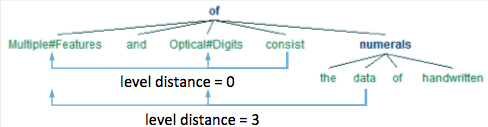
\includegraphics[width=1.05\linewidth]{figures/level-distance.png}
\caption{Dependency Tree Example}
\vspace{-0.3cm}
\label{fig:view}
\end{figure}

\subsection{CRF Feature Space}
\label{sect:pdf}

For the production of the electronic manuscript you must use Adobe's
Portable Document Format (PDF). PDF files are usually produced from
\LaTeX\ using the \textit{pdflatex} command. If your version of
\LaTeX\ produces Postscript files, you can convert these into PDF
using \textit{ps2pdf} or \textit{dvipdf}. On Windows, you can also use
Adobe Distiller to generate PDF.

Please make sure that your PDF file includes all the necessary fonts
(especially tree diagrams, symbols, and fonts with Asian
characters). When you print or create the PDF file, there is usually
an option in your printer setup to include none, all or just
non-standard fonts.  Please make sure that you select the option of
including ALL the fonts. \textbf{Before sending it, test your PDF by
  printing it from a computer different from the one where it was
  created.} Moreover, some word processors may generate very large PDF
files, where each page is rendered as an image. Such images may
reproduce poorly. In this case, try alternative ways to obtain the
PDF. One way on some systems is to install a driver for a postscript
printer, send your document to the printer specifying ``Output to a
file'', then convert the file to PDF.

It is of utmost importance to specify the \textbf{A4 format} (21 cm
x 29.7 cm) when formatting the paper. When working with
{\tt dvips}, for instance, one should specify {\tt -t a4}.

Print-outs of the PDF file on A4 paper should be identical to the
hardcopy version. If you cannot meet the above requirements about the
production of your electronic submission, please contact the
publication chairs as soon as possible.


\subsection{Layout}
\label{ssec:layout}

Format manuscripts two columns to a page, in the manner these
instructions are formatted. The exact dimensions for a page on A4
paper are:

\begin{itemize}
\item Left and right margins: 2.5 cm
\item Top margin: 2.5 cm
\item Bottom margin: 2.5 cm
\item Column width: 7.7 cm
\item Column height: 24.7 cm
\item Gap between columns: 0.6 cm
\end{itemize}

\noindent Papers should not be submitted on any other paper size.
 If you cannot meet the above requirements about the production of your electronic submission, please contact the publication chairs above as soon as possible.


\subsection{Fonts}

For reasons of uniformity, Adobe's {\bf Times Roman} font should be
used. In \LaTeX2e{} this is accomplished by putting

\begin{quote}
\begin{verbatim}
\usepackage{times}
\usepackage{latexsym}
\end{verbatim}
\end{quote}
in the preamble. If Times Roman is unavailable, use {\bf Computer
  Modern Roman} (\LaTeX2e{}'s default).  Note that the latter is about
  10\% less dense than Adobe's Times Roman font.


\begin{table}[h]
\begin{center}
\begin{tabular}{|l|rl|}
\hline \bf Type of Text & \bf Font Size & \bf Style \\ \hline
paper title & 15 pt & bold \\
author names & 12 pt & bold \\
author affiliation & 12 pt & \\
the word ``Abstract'' & 12 pt & bold \\
section titles & 12 pt & bold \\
document text & 11 pt  &\\
captions & 11 pt & \\
abstract text & 10 pt & \\
bibliography & 10 pt & \\
footnotes & 9 pt & \\
\hline
\end{tabular}
\end{center}
\caption{\label{font-table} Font guide. }
\end{table}

\subsection{The First Page}
\label{ssec:first}

Center the title, author's name(s) and affiliation(s) across both
columns. Do not use footnotes for affiliations. Do not include the
paper ID number assigned during the submission process. Use the
two-column format only when you begin the abstract.

{\bf Title}: Place the title centered at the top of the first page, in
a 15-point bold font. (For a complete guide to font sizes and styles,
see Table~\ref{font-table}) Long titles should be typed on two lines
without a blank line intervening. Approximately, put the title at 2.5
cm from the top of the page, followed by a blank line, then the
author's names(s), and the affiliation on the following line. Do not
use only initials for given names (middle initials are allowed). Do
not format surnames in all capitals (e.g., use ``Schlangen'' not
``SCHLANGEN'').  Do not format title and section headings in all
capitals as well except for proper names (such as ``BLEU'') that are
conventionally in all capitals.  The affiliation should contain the
author's complete address, and if possible, an electronic mail
address. Start the body of the first page 7.5 cm from the top of the
page.

The title, author names and addresses should be completely identical
to those entered to the electronical paper submission website in order
to maintain the consistency of author information among all
publications of the conference. If they are different, the publication
chairs may resolve the difference without consulting with you; so it
is in your own interest to double-check that the information is
consistent.

{\bf Abstract}: Type the abstract at the beginning of the first
column. The width of the abstract text should be smaller than the
width of the columns for the text in the body of the paper by about
0.6 cm on each side. Center the word {\bf Abstract} in a 12 point bold
font above the body of the abstract. The abstract should be a concise
summary of the general thesis and conclusions of the paper. It should
be no longer than 200 words. The abstract text should be in 10 point font.

{\bf Text}: Begin typing the main body of the text immediately after
the abstract, observing the two-column format as shown in 
the present document. Do not include page numbers.

{\bf Indent} when starting a new paragraph. Use 11 points for text and 
subsection headings, 12 points for section headings and 15 points for
the title. 

\subsection{Sections}

{\bf Headings}: Type and label section and subsection headings in the
style shown on the present document.  Use numbered sections (Arabic
numerals) in order to facilitate cross references. Number subsections
with the section number and the subsection number separated by a dot,
in Arabic numerals. Do not number subsubsections.

{\bf Citations}: Citations within the text appear in parentheses
as~\cite{Gusfield:97} or, if the author's name appears in the text
itself, as Gusfield~\shortcite{Gusfield:97}.  Append lowercase letters
to the year in cases of ambiguity.  Treat double authors as
in~\cite{Aho:72}, but write as in~\cite{Chandra:81} when more than two
authors are involved. Collapse multiple citations as
in~\cite{Gusfield:97,Aho:72}. Also refrain from using full citations
as sentence constituents. We suggest that instead of
\begin{quote}
  ``\cite{Gusfield:97} showed that ...''
\end{quote}
you use
\begin{quote}
``Gusfield \shortcite{Gusfield:97}   showed that ...''
\end{quote}

If you are using the provided \LaTeX{} and Bib\TeX{} style files, you
can use the command \verb|\newcite| to get ``author (year)'' citations.

As reviewing will be double-blind, the submitted version of the papers
should not include the authors' names and affiliations. Furthermore,
self-references that reveal the author's identity, e.g.,
\begin{quote}
``We previously showed \cite{Gusfield:97} ...''  
\end{quote}
should be avoided. Instead, use citations such as 
\begin{quote}
``Gusfield \shortcite{Gusfield:97}
previously showed ... ''
\end{quote}

\textbf{Please do not use anonymous citations} and do not include
acknowledgements when submitting your papers. Papers that do not
conform to these requirements may be rejected without review.

\textbf{References}: Gather the full set of references together under
the heading {\bf References}; place the section before any Appendices,
unless they contain references. Arrange the references alphabetically
by first author, rather than by order of occurrence in the text.
Provide as complete a citation as possible, using a consistent format,
such as the one for {\em Computational Linguistics\/} or the one in the 
{\em Publication Manual of the American 
Psychological Association\/}~\cite{APA:83}.  Use of full names for
authors rather than initials is preferred.  A list of abbreviations
for common computer science journals can be found in the ACM 
{\em Computing Reviews\/}~\cite{ACM:83}.

The \LaTeX{} and Bib\TeX{} style files provided roughly fit the
American Psychological Association format, allowing regular citations, 
short citations and multiple citations as described above.

{\bf Appendices}: Appendices, if any, directly follow the text and the
references (but see above).  Letter them in sequence and provide an
informative title: {\bf Appendix A. Title of Appendix}.

\subsection{Footnotes}

{\bf Footnotes}: Put footnotes at the bottom of the page and use 9
points text. They may be numbered or referred to by asterisks or other
symbols.\footnote{This is how a footnote should appear.} Footnotes
should be separated from the text by a line.\footnote{Note the line
separating the footnotes from the text.}

\subsection{Graphics}

{\bf Illustrations}: Place figures, tables, and photographs in the
paper near where they are first discussed, rather than at the end, if
possible.  Wide illustrations may run across both columns.  Color
illustrations are discouraged, unless you have verified that  
they will be understandable when printed in black ink.

{\bf Captions}: Provide a caption for every illustration; number each one
sequentially in the form:  ``Figure 1. Caption of the Figure.'' ``Table 1.
Caption of the Table.''  Type the captions of the figures and 
tables below the body, using 11 point text.


\section{XML conversion and supported \LaTeX\ packages}

ACL 2014 innovates over earlier years in that we will attempt to
automatically convert your \LaTeX\ source files to machine-readable
XML with semantic markup. This will facilitate future research that
uses the ACL proceedings themselves as a corpus.

We encourage you to submit a ZIP file of your \LaTeX\ sources along
with the camera-ready version of your paper. We will then convert them
to XML automatically, using the LaTeXML tool
(\url{http://dlmf.nist.gov/LaTeXML}). LaTeXML has \emph{bindings} for
a number of \LaTeX\ packages, including the ACL 2014 stylefile. These
bindings allow LaTeXML to render the commands from these packages
correctly in XML. For best results, we encourage you to use the
packages that are officially supported by LaTeXML, listed at
\url{http://dlmf.nist.gov/LaTeXML/manual/included.bindings}





\section{Translation of non-English Terms}

It is also advised to supplement non-English characters and terms
with appropriate transliterations and/or translations
since not all readers understand all such characters and terms.
Inline transliteration or translation can be represented in
the order of: original-form transliteration ``translation''.

\section{Length of Submission}
\label{sec:length}

Long papers may consist of up to 9 pages of content, plus two extra
pages for references. Short papers may consist of up to 5 pages of
content, plus two extra pages for references.  Papers that do not
conform to the specified length and formatting requirements may be
rejected without review.



\section*{Acknowledgments}

The acknowledgments should go immediately before the references.  Do
not number the acknowledgments section. Do not include this section
when submitting your paper for review.

% include your own bib file like this:
%\bibliographystyle{acl}
%\bibliography{acl2014}

\begin{thebibliography}{}

\bibitem[\protect\citename{Aho and Ullman}1972]{Aho:72}
Alfred~V. Aho and Jeffrey~D. Ullman.
\newblock 1972.
\newblock {\em The Theory of Parsing, Translation and Compiling}, volume~1.
\newblock Prentice-{Hall}, Englewood Cliffs, NJ.

\bibitem[\protect\citename{{American Psychological Association}}1983]{APA:83}
{American Psychological Association}.
\newblock 1983.
\newblock {\em Publications Manual}.
\newblock American Psychological Association, Washington, DC.

\bibitem[\protect\citename{{Association for Computing Machinery}}1983]{ACM:83}
{Association for Computing Machinery}.
\newblock 1983.
\newblock {\em Computing Reviews}, 24(11):503--512.

\bibitem[\protect\citename{Chandra \bgroup et al.\egroup }1981]{Chandra:81}
Ashok~K. Chandra, Dexter~C. Kozen, and Larry~J. Stockmeyer.
\newblock 1981.
\newblock Alternation.
\newblock {\em Journal of the Association for Computing Machinery},
  28(1):114--133.

\bibitem[\protect\citename{Gusfield}1997]{Gusfield:97}
Dan Gusfield.
\newblock 1997.
\newblock {\em Algorithms on Strings, Trees and Sequences}.
\newblock Cambridge University Press, Cambridge, UK.

\end{thebibliography}

\end{document}
